\documentclass[a4paper, 12pt]{article}%тип документа



%отступы
\usepackage[left=1cm,right=1cm,top=1cm,bottom=2cm,bindingoffset=0cm]{geometry}

%%% Работа с русским языком
\usepackage{graphicx}
\usepackage{cmap}                           % поиск в PDF
\usepackage{mathtext} 			 	       % русские буквы в формулах
\usepackage[T2A]{fontenc}               % кодировка
\usepackage[utf8]{inputenc}              % кодировка исходного текста
\usepackage[english,russian]{babel} 
\usepackage{float}

\usepackage[export]{adjustbox} % локализация и переносы

\usepackage{subfig}% http://ctan.org/pkg/subfig
\usepackage{booktabs}

\usepackage{wrapfig}


%Матеша
\usepackage{amsmath,amsfonts,amssymb,amsthm,mathtools} % AMS
\usepackage{icomma} % "Умная" запятая

%\mathtoolsset{showonlyrefs=true} % Показывать номера только у тех формул, на которые есть \eqref{} в тексте.

%% Шрифты
\usepackage{euscript}	 % Шрифт Евклид
\usepackage{mathrsfs} % Красивый матшрифт

%% Свои команды
\DeclareMathOperator{\sgn}{\mathop{sgn}}

%% Перенос знаков в формулах (по Львовскому)
\newcommand*{\hm}[1]{#1\nobreak\discretionary{}
	{\hbox{$\mathsurround=0pt #1$}}{}}




\author{Гаврилин Илья Дмитриевич \\
	Б01-101}
\title{\textbf{Работа 2.1.4 \\ 
		Определение теплоемкости твердых тел}}

\begin{document}
	\maketitle
	\section{Аннотация}
	В данной работе производится измерение теплоемкости твердых тел $C$ (усеченных конусов из латуни и алюминия). В ходе работы получена зависимость температуры тела от времени, при условии постоянной мощности нагрева. Также, оценены и учтены, при расчете теплоемкости, тепло потери калориметра. Оценены погрешности измеряемых величин.
	\section{Сведения о работе}
	\subsection{Теоретические сведения}
	В данной работе происходит измерение теплоемкости твердого тела с использованием следующей принципиальной связи:
	
	\begin{equation}
		C = \frac{\Delta Q}{\Delta T}
		\label{eq:first_eq_of_thermal_capacity}
	\end{equation}
	
	Определение количества теплоты, переданного телу вызывает некоторые затруднения, так как часть теплоты будет передано окружающей среде через стенки калориметра. В итоге, количество теплоты, переданное телу с учетом теплопотерь через стенки можно определить как:
	
	\begin{equation}
		\Delta Q = P\Delta t - \lambda \left( T - T_{\text{к}} \right) \Delta t,
		\label{eq:termal_with_heat_lossing}
	\end{equation}
	где $P$ -- мощность нагревателя, $\lambda$ -- коэффициент теплоотдачи стенок калориметра, $T$ -- температура тела, $T_{\text{к}}$ -- температура окружающего калориметр воздуха, $\Delta t$ -- время, в течении которого происходит нагрев.
	
	Из уравнений (\ref{eq:first_eq_of_thermal_capacity}) и (\ref{eq:second_eq_of_thremal_capacity}) получаем:
	
	\begin{equation}
		C = \frac{P - \lambda \left(T - T_{\text{к}} \right) }{\Delta T /\Delta t}
		\label{eq:second_eq_of_thremal_capacity}
	\end{equation}
	
	Формула (\ref{eq:second_eq_of_thremal_capacity}) является основной расчетной формулой данной работы.
	
	В формуле (\ref{eq:second_eq_of_thremal_capacity} в знаменателе стоит величина, для определения которой воспользуемся следующей методикой:
	
	Построим график зависимости $\frac{\Delta T}{\Delta t} = f \left( T \right)$ для широкого диапазона температур, после чего экстраполируем его для значения $T = T_{\text{к}}$. В таком случае формула (\ref{eq:second_eq_of_thremal_capacity}) приобретает вид:
	
	\begin{equation}
		C = \frac{P}{\left( \Delta T / \Delta t \right)_{T_{\text{к}}}}
		\label{eq:final_eq_for_capacity}
	\end{equation}
	
	Измерение температуры строится на принципе линейной зависимости сопротивления материала от изменения температуры по закону:
	
	\begin{equation}
		R_{T} = R_{0} \left( 1 + \alpha \Delta T \right),
	\end{equation}
	
	Где $R_{0}$ -- сопротивление термометра при комнатной температуры, $R_{T}$ -- сопротивление термометра при данной температуре. Учитывая данную зависимость, получаем итоговый вид для основной формулы:
	
	\begin{equation}
		C = \frac{PR\alpha}{\left( \frac{dR}{dt} \right)_{T_{\text{к}}}\left( 1 + \alpha \Delta T_{\text{К}} \right)}
		\label{eq:capacity}
	\end{equation}	 
	
	Коэффициент $\alpha$, входящий в данную формулу для меди равен $\alpha = 4,28 \cdot 10^{-3} \, K^{-1}$, все остальные величины определяются экспериментально.
	\subsection{Схема установки}
	Установка состоит из сосуда формы усеченного конуса, для более плотного прилегания измеряемого тела к сосуду. Он снабжен спиралью нагревателя постоянной мощности: $ U = 36 \, \text{В}, \, I = 0,6 \, \text{А}, \, P = 10,8 \, \text{Вт} $ . \\
	\begin{figure}[H]
		\centering
		\includegraphics[width=0.6\linewidth]{"Снимок экрана 2022-03-30 222759"}
		\caption{Схема калориметра}
	\end{figure}
	Параметры экспериментальной установки: $ R_{0} = 18.155 \pm 0.01 \, \text{Ом}, \, t = 23 \pm 1~ C^{o}$. Запишем массы измеряемых тел.
	\begin{table}[H]
		\centering
		\begin{tabular}{|c|c|c|c|}
			\hline
			материал образца: & железо          & латунь          & алюминий        \\ \hline
			масса образца, г  & $815,1 \pm 0,1$ & $875,5 \pm 0,1$ & $294,2 \pm 0,1$ \\ \hline
		\end{tabular}
		\caption{Массы исследуемых образцов}

	\end{table}
	\section{Ход работы}
	\subsection{Зависимость R(t)}
	Включим магазин сопротивлений согласно приложенной инструкции, включим нагрев постоянной мощности, начнем замеры. Будем замерять сколько пройдет времени до установки определенного значения сопротивления терморезистора (разница в сопротивлениях $\Delta R = 0.05 ~ Ом$)
	
	\begin{table}[H]
		\centering
		\begin{tabular}{|cc|cc|cc|}
			\hline
			\multicolumn{2}{|c|}{Пустой   калориметр} & \multicolumn{2}{c|}{Латунь}          & \multicolumn{2}{c|}{алюминий}      \\ \hline
			\multicolumn{1}{|c|}{R, Ом}    & T, сек   & \multicolumn{1}{c|}{R, Ом}  & T, сек & \multicolumn{1}{c|}{R, Ом}  & T, сек \\ \hline
			\multicolumn{1}{|c|}{18.155}   & 0.00     & \multicolumn{1}{c|}{18.155} & 0.00   & \multicolumn{1}{c|}{18.155} & 0.00   \\ \hline
			\multicolumn{1}{|c|}{18.205}   & 18.15    & \multicolumn{1}{c|}{18.205} & 62.15  & \multicolumn{1}{c|}{18.205} & 53.23  \\ \hline
			\multicolumn{1}{|c|}{18.255}   & 62.81    & \multicolumn{1}{c|}{18.255} & 129.01 & \multicolumn{1}{c|}{18.255} & 111.58 \\ \hline
			\multicolumn{1}{|c|}{18.305}   & 107.21   & \multicolumn{1}{c|}{18.305} & 198.25 & \multicolumn{1}{c|}{18.305} & 173.24 \\ \hline
			\multicolumn{1}{|c|}{18.355}   & 153.62   & \multicolumn{1}{c|}{18.355} & 271.86 & \multicolumn{1}{c|}{18.355} & 237.32 \\ \hline
			\multicolumn{1}{|c|}{18.405}   & 201.22   & \multicolumn{1}{c|}{18.405} & 344.93 & \multicolumn{1}{c|}{18.405} & 302.36 \\ \hline
			\multicolumn{1}{|c|}{18.455}   & 252.34   & \multicolumn{1}{c|}{18.455} & 418.38 & \multicolumn{1}{c|}{18.455} & 375.81 \\ \hline
			\multicolumn{1}{|c|}{18.505}   & 304.69   & \multicolumn{1}{c|}{18.505} & 498.56 & \multicolumn{1}{c|}{18.505} & 443.00 \\ \hline
			\multicolumn{1}{|c|}{18.555}   & 355.25   & \multicolumn{1}{c|}{18.555} & 588.46 & \multicolumn{1}{c|}{18.555} & 517.12 \\ \hline
			\multicolumn{1}{|c|}{18.605}   & 414.20   & \multicolumn{1}{c|}{18.605} & 659.37 & \multicolumn{1}{c|}{18.605} & 591.08 \\ \hline
			\multicolumn{1}{|c|}{18.655}   & 465.56   & \multicolumn{1}{c|}{18.655} & 747.68 & \multicolumn{1}{c|}{18.655} & 667.77 \\ \hline
		\end{tabular}
	\caption{Зависимость сопротивления от времени}
	\end{table}
	По полученным зависимостям сопротивления проволоки от времени построим графики зависимости $R(t)$ и экстраполируем их полиномом третьей степени ($R(t) = at^{3} + bt^{2} + ct + d$) Коэффициенты полученные в ходе экстраполяции указаны на графиках.
	\begin{figure}[H]
		\begin{center}
			\begin{minipage}[h]{0.48\linewidth}
				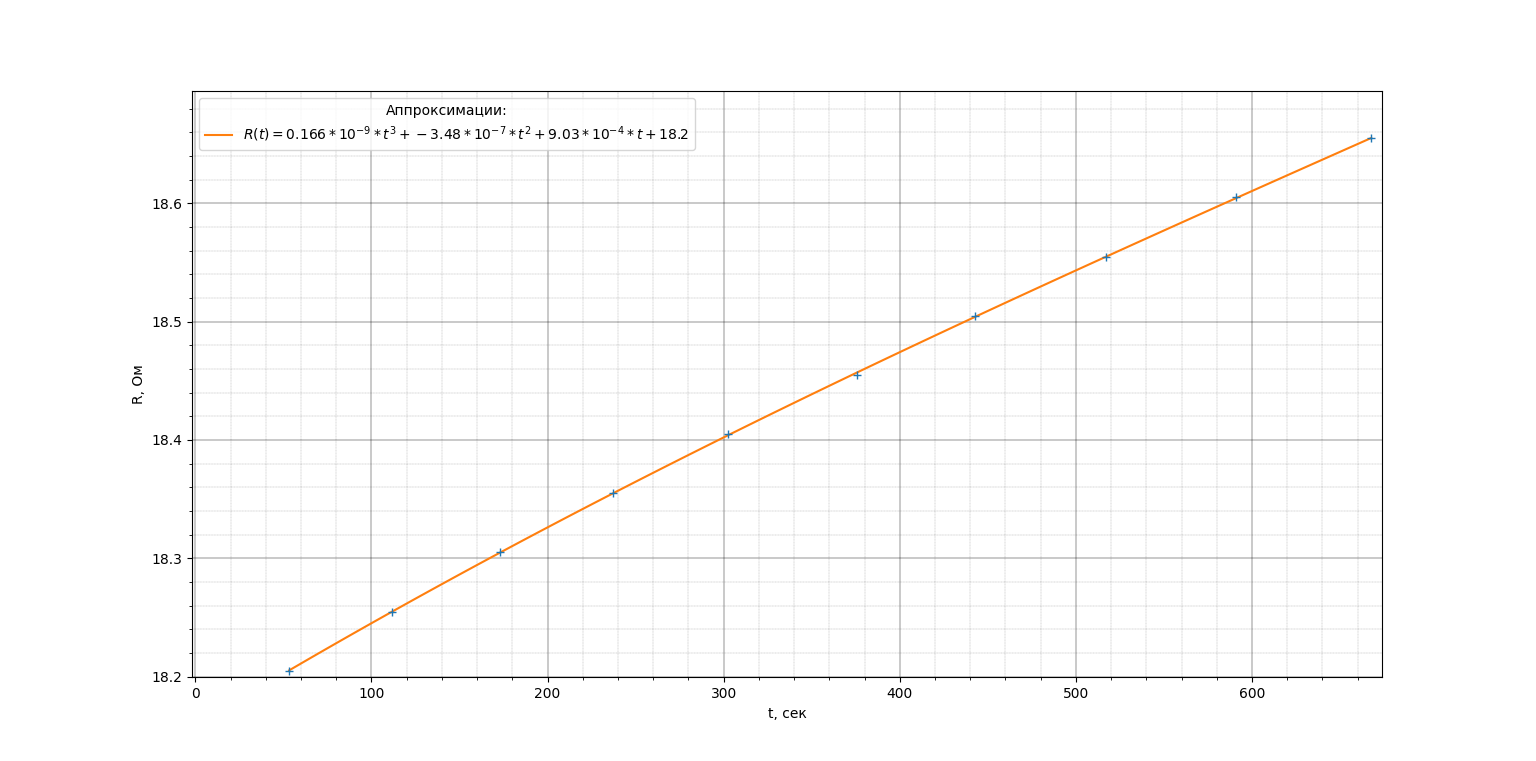
\includegraphics[width=1\linewidth]{graph_al}
				\caption{Зависимость $R(t)$ для алюминия} %% подпись к рисунку
			\end{minipage}
			\hfill
			\begin{minipage}[h]{0.48\linewidth}
				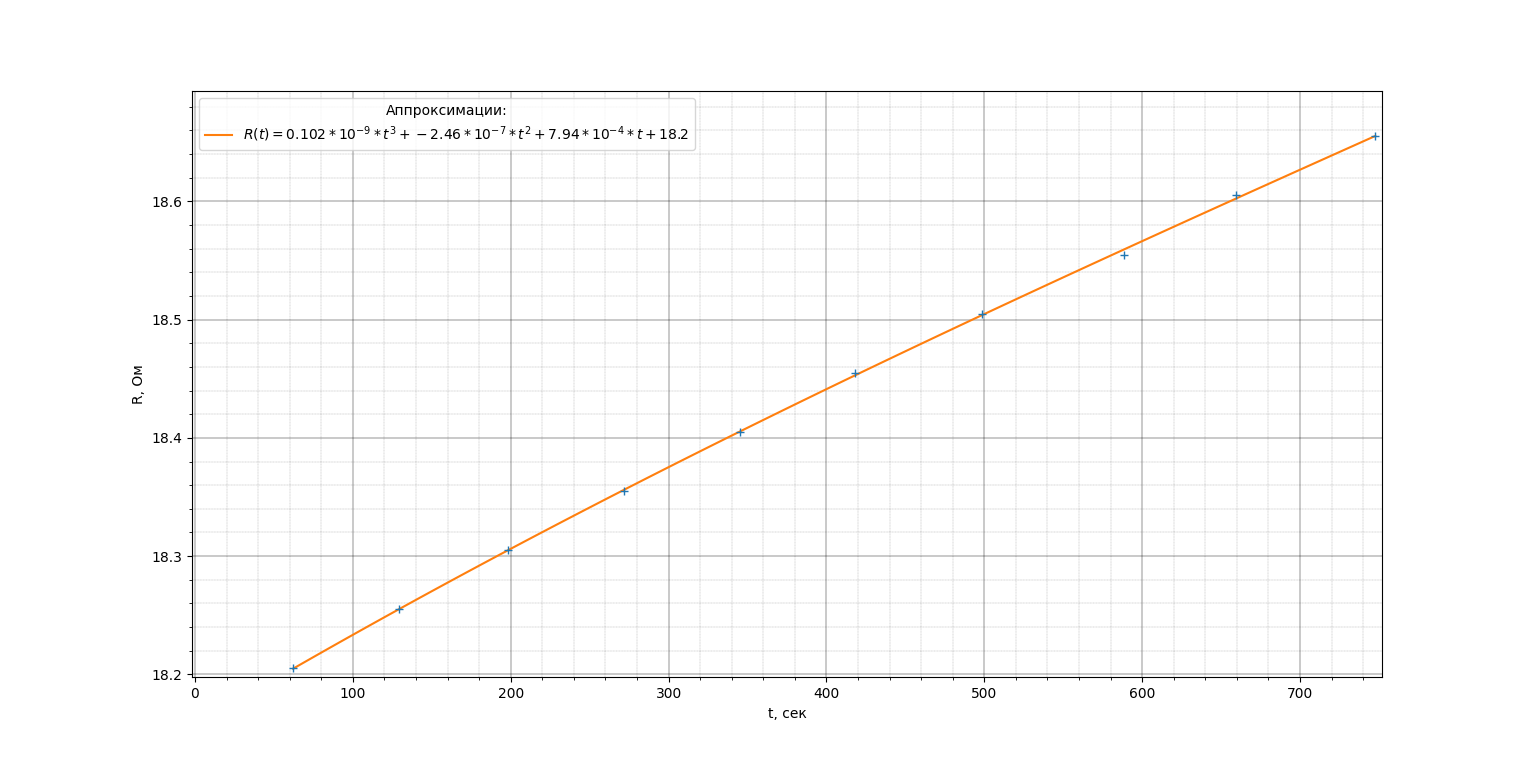
\includegraphics[width=1\linewidth]{graph_lat}
				\caption{Зависимость $R(t)$ для латуни}
				

			\end{minipage}

		\end{center}
		\begin{center}
			\begin{minipage}[h]{0.98\linewidth}
				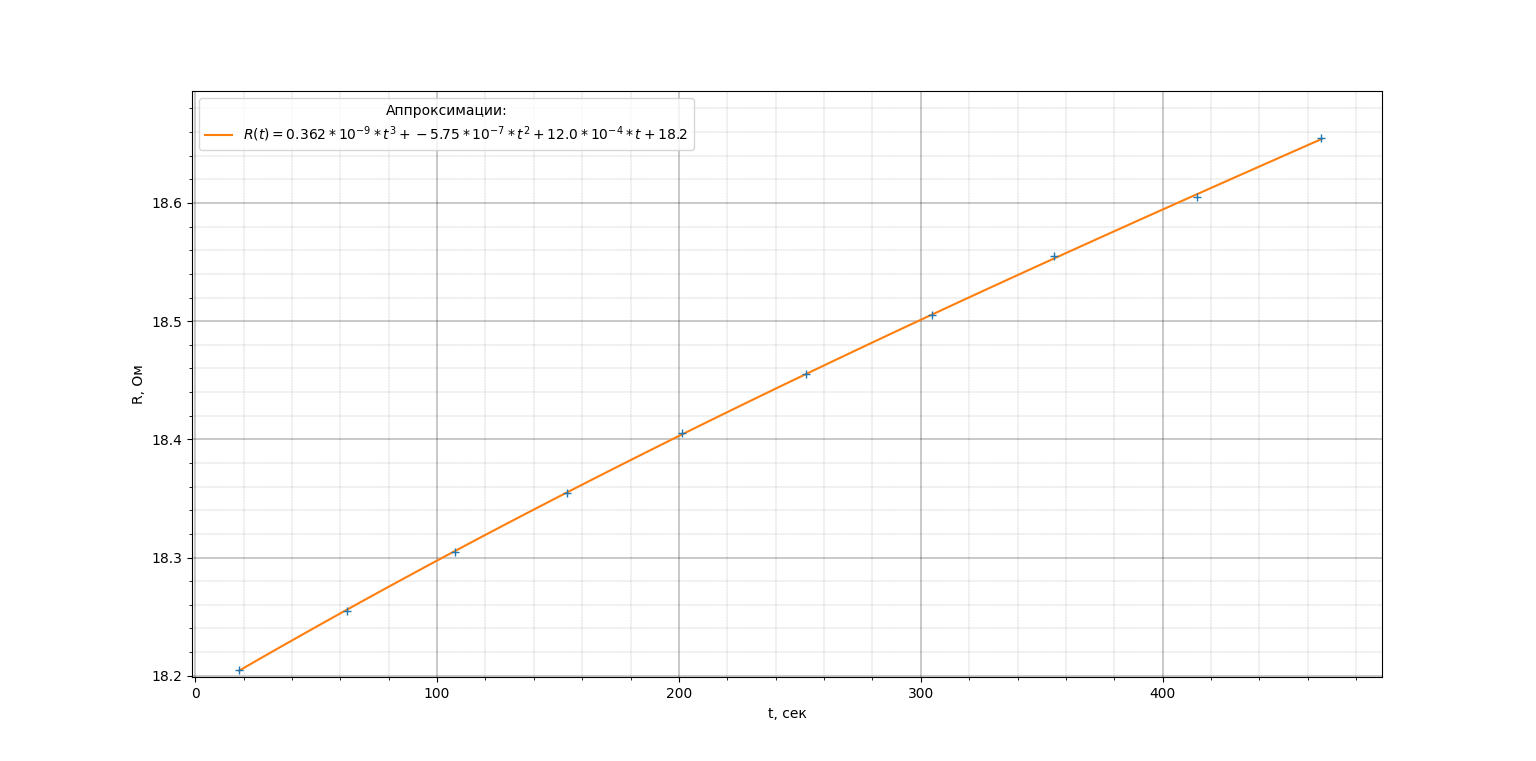
\includegraphics[width=1\linewidth]{graph_empty}
				\caption{Зависимость $R(t)$ для калориметра}
			\end{minipage}
		\end{center}
	\end{figure}
	\subsection{Зависимость $\frac{dR}{dt}(R)$}
	В прошлом пункте получили зависимость R(t), дифференцируя ее получим функцию $\frac{dR}{dt}(t)$. Однако мы знаем связь между сопротивлением и временем и меняя переменную получим $\frac{dR}{dt}(R)$. По полученной аппроксимации для каждого опыта вычислим $\frac{dR}{dt}(R_{к})$. Для большей наглядности на графиках отмечены точки полученные наивным дифференцированием:
	\begin{equation}
		\frac{dR}{dt} \left( R_{t_{1}} \right) = \frac{R_{t_{2}} - R_{t_{2}}}{t_{2} - t_{1}}
		\label{eq:derivates}
	\end{equation}
		\begin{figure}[H]
		\begin{center}
			\begin{minipage}[h]{0.48\linewidth}
				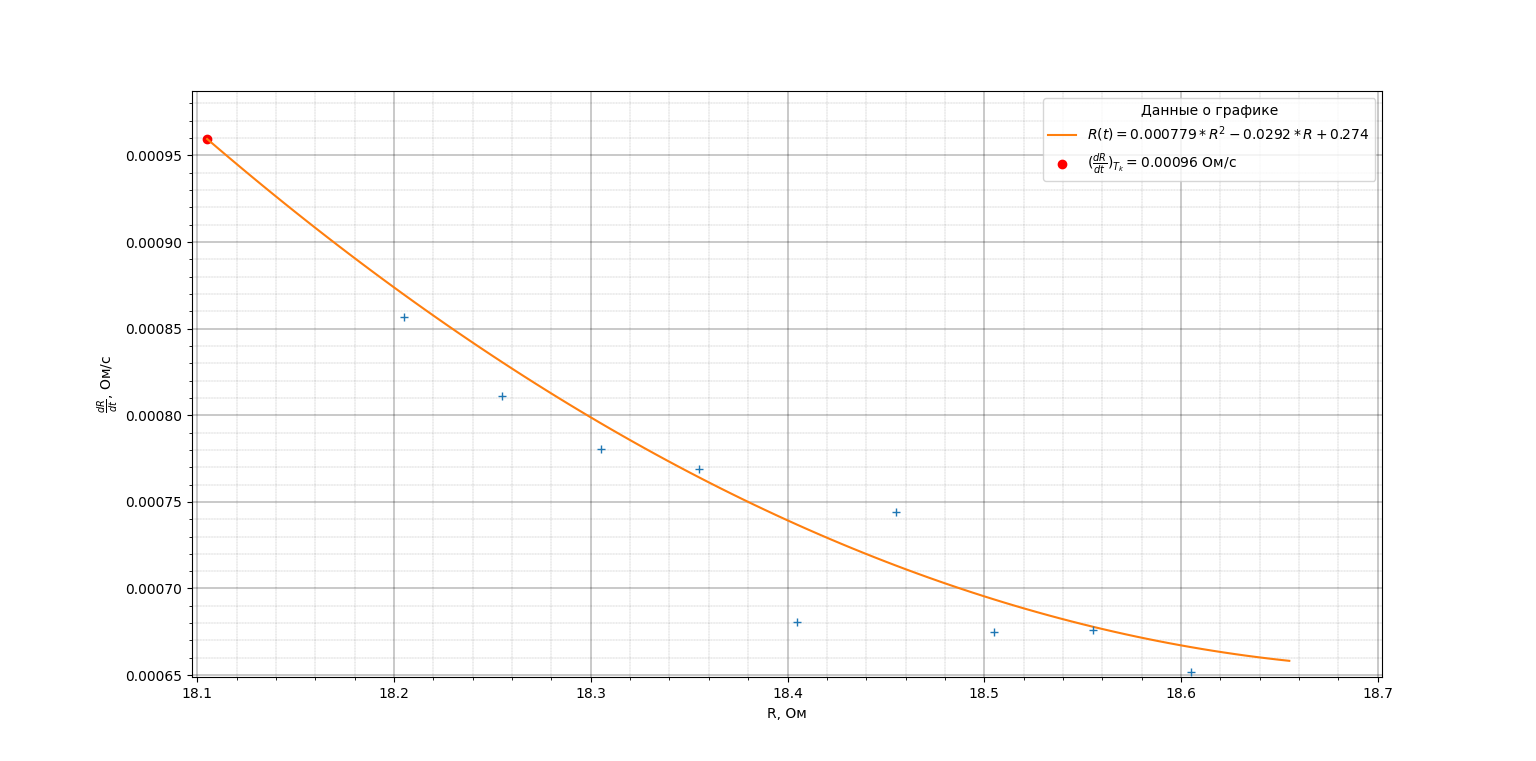
\includegraphics[width=1\linewidth]{deriv_al}
				\caption{Зависимость $\frac{dR}{dt}(R)$ для алюминия} %% подпись к рисунку
			\end{minipage}
			\hfill
			\begin{minipage}[h]{0.48\linewidth}
				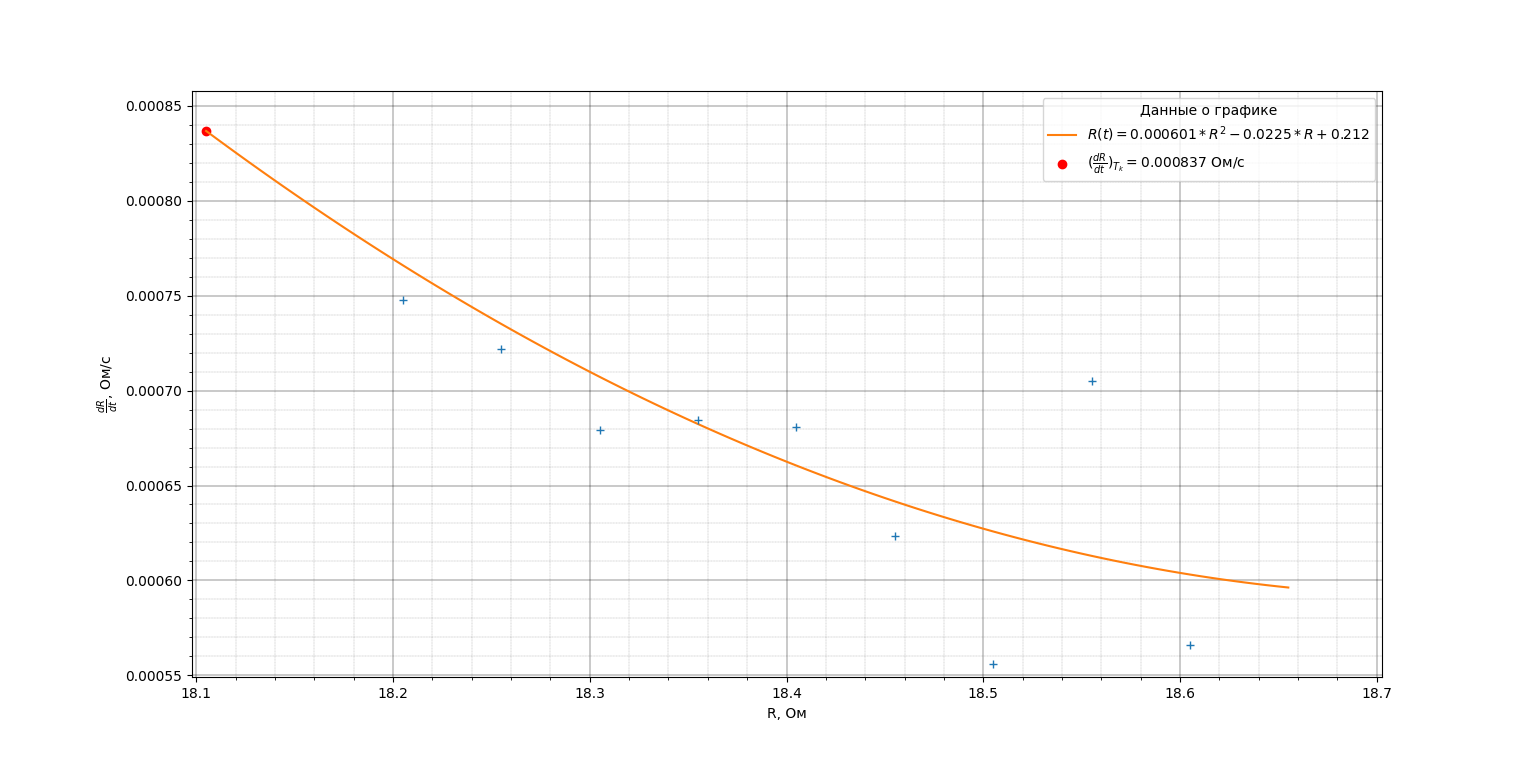
\includegraphics[width=1\linewidth]{deriv_lat}
				\caption{Зависимость $\frac{dR}{dt}(R)$ для латуни}
				
				
			\end{minipage}
			
		\end{center}
		\begin{center}
			\begin{minipage}[h]{0.98\linewidth}
				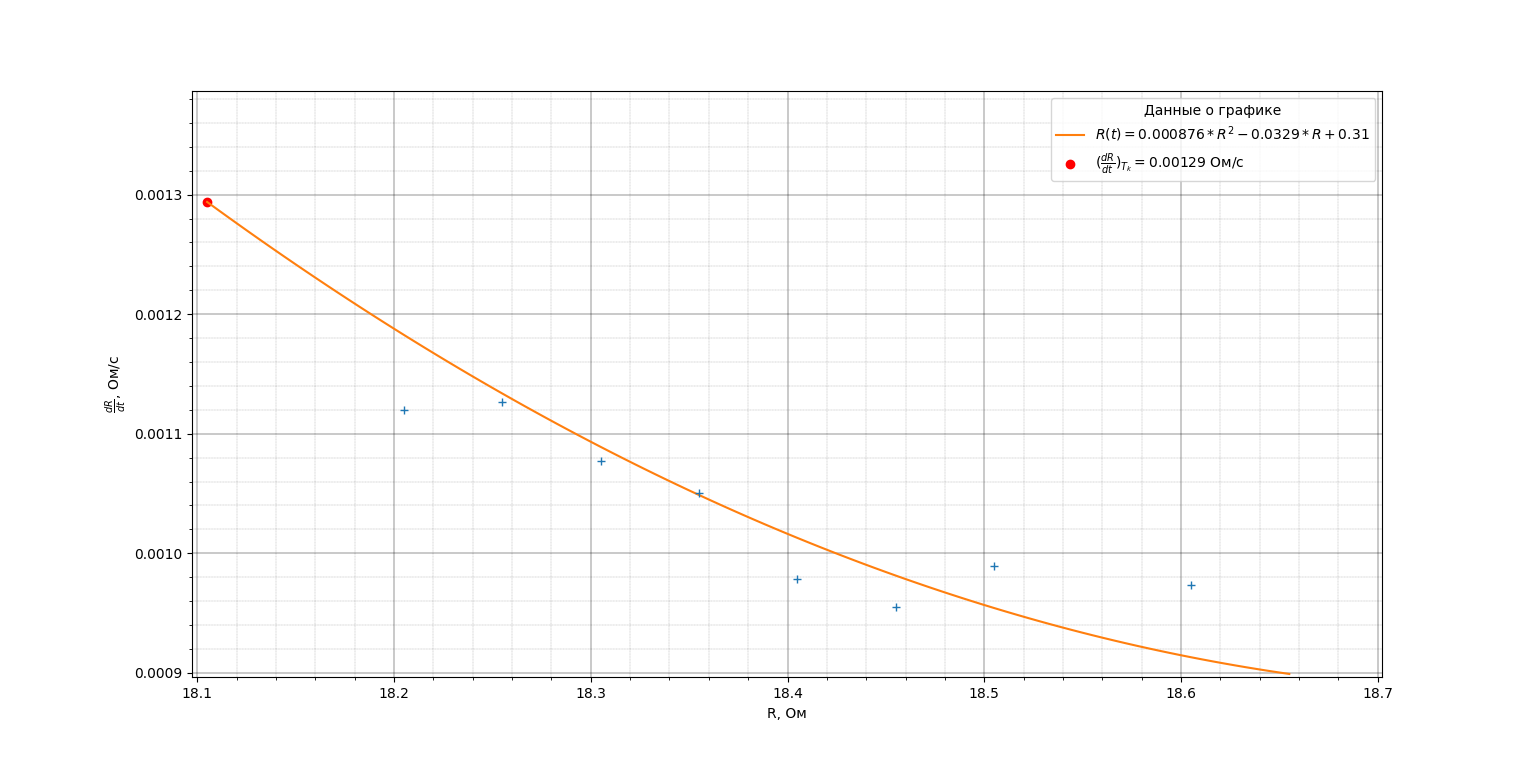
\includegraphics[width=1\linewidth]{deriv_empty}
				\caption{Зависимость $\frac{dR}{dt}(R)$ для калориметра}
			\end{minipage}
		\end{center}
	\end{figure}
	Подставляя $R_{K} = 18,155 \, \text{Ом}$, определяем значения $\frac{dR}{dt} \left( R_{K} \right)$. Результаты занесем в таблицу 3.
	
	\begin{table}[H]
		\centering
		\begin{tabular}{|c|c|}
			\hline
			исследуемое тело & $\frac{dR}{dt} \left( R_{K} \right)$, $\frac{\text{Ом}}{\text{с}} \cdot 10^{-4}$ \\ \hline
			калориметр          & 12,9 \\ \hline
			латунный образец    & 8,4  \\ \hline
			алюминиевый образец & 9,6  \\ \hline
		\end{tabular}
		\caption{Значения $\frac{dR}{dt} \left( R_{K} \right)$ для различных образцов}
	\end{table}
	
	Для определения теплоемкости, как видно из формулы (\ref{eq:capacity}), необходимо определить разность температур для каждого значения сопротивления. Очевидно, что разность температур не зависит от исследуемого материала для каждого значения сопротивления $R$. Тогда достаточно провести измерения для одной серии измерений. Зависимость разницы температур $\Delta T$ от $R$ задается следующей формулой:
	
	\begin{equation}
		\Delta T = \frac{R_{T} - R_{K}}{R_{K} \cdot \alpha}
	\end{equation}
	
	Результаты занесем в таблицу 4.
	
	\begin{table}[H]
		\centering
		\begin{tabular}{|c|c|c|c|c|c|c|c|c|c|c|}
			\hline
			R, Ом         & 18,205   & 18,255   & 18,305   & 18,355   & 18,405   & 18,455   & 18,505   & 18,555  & 18,605 & 18,655 \\ \hline
			$\Delta T$, К & 0,643 & 1,287 & 1,931 & 2,574 & 3,217 & 3,861 & 4,504 & 5,148 & 5,791 & 6,435\\ \hline
			
		\end{tabular}
		\caption{Зависимость разницы температур от сопротивления термометра.}
		\label{tab:diffrence_between_temperature}
	\end{table}
		Тогда по формуле (6) получим результаты для теплоемкостей и вычтя теплоемкость калориметра получим теплоемкость объектов.
	\begin{table}[h!]
		\centering
		\begin{tabular}{|c|c|}
			\hline
			исследуемое тело                 & $C, \frac{\text{Дж}}{\text{К}}$  \\ \hline
			калориметр                       & 649 \\ \hline	
			калориметр + латунный образец    & 972 \\ \hline
			калориметр + алюминиевый образец & 916 \\ \hline
		\end{tabular}
		\caption{Результаты вычисления теплоемкостей}
		\label{tab:first_results_for_capacity}
	\end{table}
	\begin{figure}[H]
		\begin{center}
			\begin{minipage}[h]{0.48\linewidth}
				\centering
				\begin{tabular}{|c|c|}
					\hline
					исследуемое тело                 & $C, \frac{\text{Дж}}{\text{К}}, $  \\ \hline
					калориметр                       & 649 \\ \hline	
					латунный образец   				 & 323 \\ \hline
					алюминиевый образец 			 & 267 \\ \hline
				\end{tabular}
				\caption{Результаты вычисления теплоемкостей}
			\end{minipage}
			\hfill
			\begin{minipage}[h]{0.48\linewidth}
				\centering
				\begin{tabular}{|c|c|}
					\hline
					исследуемое тело                 & $C, \frac{\text{Дж}}{\text{кг*К}}, $  \\ \hline
					латунный образец   				 & 369 \\ \hline
					алюминиевый образец 			 & 908 \\ \hline
				\end{tabular}
				\caption{Результаты вычисления теплоемкостей}
			\end{minipage}
			
		\end{center}
	\end{figure}
	\begin{table}[h!]
		
		\label{tab:second_results_for_capacity}
	\end{table}

	\begin{table}[H]
		

	\end{table}
	\begin{center}
		Итоговые значения определенных величин:
	\end{center}
	
	\begin{table}[H]
		\centering
		\begin{tabular}{|c|c|c|}
			\hline
			исследуемое тело & $C, \frac{\text{Дж}}{\text{К}}$ & $c, \frac{\text{Дж}}{\text{кг К}}$ \\ \hline
			калориметр          & $649 \pm 68 $ & --            \\ \hline
			латунный образец    & $323 \pm 12 $ & $369 \pm 8 $  \\ \hline
			алюминиевый образец & $257 \pm 17 $ & $908 \pm 59 $ \\ \hline
		\end{tabular}
		\caption{Итоговые значения определяемых величин.}
	\end{table}
	\section{Вывод}
	1.В ходе работы были получены значения теплоемкостей разных материалов. (см. таблицу 8). Значения для латуни и алюминия совпадают с табличными в пределах погрешности. 
	2. Основные погрешности при измерении возникли из-за экстраполяции графиков, и перехода от временной зависимости к зависимости от сопротивления.
\end{document}
